\section[More]{Core modern \cpp}

\subsection[const]{Constness}

\begin{frame}[fragile]
  \frametitlecpp[98]{Constness}
  \begin{block}{The {\it const} keyword}
    \begin{itemize}
    \item indicate that the element to the left is constant
    \item this element won't be modifiable in the future
    \item this is all checked at compile time
    \end{itemize}
  \end{block}
  \begin{cppcode}
    // standard syntax
    int const i = 6;

    // error : i is constant
    i = 5;

    // also ok, when nothing on the left,
    // const applies to the element on the right
    const int j = 6;
  \end{cppcode}
\end{frame}

\begin{frame}[fragile]
  \frametitlecpp[98]{Constness and pointers}
  \scriptsize
  \begin{cppcode}
    // pointer to a constant integer
    int a = 1, b = 2;
    int const *i = &a;
    *i = 5; // error, int is const
    i = &b; // ok, pointer is not const

    // constant pointer to an integer
    int * const j = &a;
    *j = 5; // ok, value can be changed
    j = &b; // error, pointer is const

    // constant pointer to a constant integer
    int const * const k = &a;
    *k = 5; // error, value is const
    k = &b; // error, pointer is const

    // const reference
    int const & l = a;
    l = b; // error, reference is const
  \end{cppcode}
\end{frame}

\begin{frame}[fragile]
  \frametitlecpp[98]{Method constness}
  \begin{block}{The {\it const} keyword for class functions}
    \begin{itemize}
    \item indicate that the function does not modify the object
    \item in other words, {\it this} is a pointer to constant object
    \end{itemize}
  \end{block}
  \begin{cppcode}
    struct Example {
      void foo() const  {
        m_member = 0; // Error : function is constant
      }
      int m_member;
    };
  \end{cppcode}
\end{frame}

\begin{frame}[fragile]
  \frametitlecpp[98]{Method constness}
  \begin{block}{Constness is part of the type}
    \begin{itemize}
    \item const T and T are different types
    \item however, T is automatically cast to const T when needed
    \end{itemize}
  \end{block}
  \begin{cppcode}
    void func(int & a);
    void funcConst(int const & a);

    int a = 0;
    int const b = 0;

    func(a);      // ok
    func(b);      // error
    funcConst(a); // ok
    funcConst(b); // ok
  \end{cppcode}
\end{frame}

\begin{frame}[fragile]
  \frametitlecpp[98]{constness}
  \begin{alertblock}{Exercise Time}
    \begin{itemize}
    \item go to code/constness
    \item open constplay.cpp
    \item try to find out which lines won't compile
    \item check your guesses by compiling for real
    \end{itemize}
  \end{alertblock}
\end{frame}

\subsection[cstexpr]{Constant Expressions}

\begin{frame}[fragile]
  \frametitlecpp[11]{Generalized Constant Expressions}
  \begin{block}{Reason of being}
    \begin{itemize}
    \item compute constant expressions at compile time
    \item even if non trivial
    \end{itemize}
  \end{block}
  \pause
  \begin{exampleblock}{Example}
    \begin{cppcode*}{}
      constexpr int f(int x) {
        return x > 1 ? x * f(x - 1) : 1;
      }
      constexpr int a = f(5); // computed at compile time
    \end{cppcode*}
  \end{exampleblock}
  \pause
  \begin{exampleblock}{Example with \cpp14}
    \begin{cppcode*}{}
      constexpr int f(int x) {
        if (x > 1) return x * f(x - 1);
        return 1;
      }
      constexpr int a = f(5); // computed at compile time
    \end{cppcode*}
  \end{exampleblock}
\end{frame}

\begin{frame}[fragile]
  \frametitlecpp[11]{Static Assertions}
  \begin{block}{static\_assert declaration}
    \begin{itemize}
    \item Performs compile time assertions; meaning a failed assertion stops compilation
    \item The expression has to be a constexpr boolean expression
    \item Purely evaluated at compile time, no effect at runtime
    \item Often used in template programming to make assertion on types, can be
      used to validate boolean compile time expressions
    \end{itemize}
  \end{block}
  \pause
  \begin{exampleblock}{Example}
    \begin{cppcode*}{}
      constexpr int f(int x) {
        return x > 1 ? x * f(x - 1) : 1;
      }
      static_assert(f(5)==120,"Expected f(5) to be 120!");
    \end{cppcode*}
  \end{exampleblock}
\end{frame}


\begin{frame}[fragile]
  \frametitlecpp[14]{Generalized Constant Expressions(2)}
   \begin{alertblock}{Few limitations in C++14 (more in C++11)}
    \begin{itemize}
    \item function's body cannot contain try-catch or static variables
    \item arguments should be constexpr or literals in order to benefit from compile time computation
    \end{itemize}
  \end{alertblock}
  \begin{block}{Notes}
    \begin{itemize}
    \item classes can have constexpr functions
    \item objects can be constexpr
      \begin{itemize}
      \item if the constructor of their class is
      \end{itemize}
    \item a constexpr function can also be used normally
    \item but a constexpr variable has to be evaluated at compile time
    \end{itemize}
  \end{block}
\end{frame}

\begin{frame}[fragile]
  \frametitlecpp[11]{Real life example}
  \begin{cppcode*}{}
    constexpr float toSI(const float v, const char unit) {
      switch (unit) {
      case 'k': return 1000*v;
      case 'm': return 0.001*v;
      case 'y': return 0.9144*v;
      case 'i': return 0.0254*v;
      ...
      default: return v;
      }
    }
    constexpr float fromSI(const float v, const char unit) {
      switch (unit) {
        case 'k': return 0.001*v;
        case 'y': return 1.093*v;
      ...
      }
    }
  \end{cppcode*}
\end{frame}

\begin{frame}[fragile]
  \frametitlecpp[11]{Real life example(2)}
  \begin{cppcode*}{}
    class DimLength {
      const float m_value;
    public:
      constexpr DimLength(const float v, const char unit):
        m_value(toSI(v, unit)) {
      }
      constexpr float get(const char unit) const {
        return fromSI(m_value, unit);
      }
    };
    constexpr DimLength km(1, 'k');
    constexpr float km_y = km.get('y');
    constexpr float km_i = km.get('i');
    static_assert(km_y == 1093, "expected km == 1093 yards!");
  \end{cppcode*}
\end{frame}

\subsection[except]{Exceptions}

\begin{frame}[fragile]
  \frametitlecpp[98]{Exceptions}
  \begin{block}{The concept}
    \begin{itemize}
    \item exceptional event breaking linearity of the code
    \item will be handled in dedicated place
    \end{itemize}
  \end{block}
  \begin{block}{Practically}
    \begin{itemize}
    \item you can throw any object with {\it throw}
    \item you handle them using {\it try ... catch} blocks
    \end{itemize}
  \end{block}
  \begin{cppcode}
    try {
      if (0 == name) {
        throw std::string("Expected non empty name");
      }
      printf("%s\n", name);
    } catch (std::string& e) {
      printf("empty name found\n");
    }
  \end{cppcode}
\end{frame}

\begin{frame}[fragile]
  \frametitlecpp[98]{Exceptions}
  \begin{block}{Rules}
    \begin{itemize}
    \item exception will skip all code until next {\it catch}
    \begin{itemize}
      \item still destructors are called when exiting scopes
      \item but your own cleanup may not be
    \end{itemize}
    \item {\it catch} is selective on the exception type
    \end{itemize}
  \end{block}
  \begin{multicols}{2}
    \begin{cppcode*}{fontsize=\scriptsize,gobble=2}
      struct ZeroDivide {};

      int divide(int a, int b) {
        if (0 == b) {
          throw ZeroDivide();
        }
        return a/b;
      }
    \end{cppcode*}
    \columnbreak
    \begin{cppcode*}{fontsize=\scriptsize,gobble=2,firstnumber=9}
      int func(char* value) {
        try {
          errno = 0;
          long l = strtol(value,0,10);
          if (errno) {
            throw string("Bad Value");
          }
          divide(100, l);
        } catch (string& e) {
          printf("%s\n", e.c_str());
        } catch (ZeroDivide e2) {
          printf("Division error\n");
        }
      }
    \end{cppcode*}
  \end{multicols}
\end{frame}

\begin{frame}[fragile]
  \frametitlecpp[98]{Controlling exceptions \hfill \deprecated/\removed}
  \begin{block}{Declaring expected exceptions}
    \begin{itemize}
    \item each function can declare a set of expected exceptions
    \item using the {\it throw} statement in its declaration
    \item other exceptions won't exit the scope of the function
      \begin{itemize}
      \item instead, the {\it unexpected} handler is called
      \item by default, it terminates the program
      \end{itemize}
    \end{itemize}
  \end{block}
  \pause
  \begin{cppcode}
    int func(int a) throw(int) {
      if (0 == a) {
        throw 2;  // ok, goes out
      } else {
        throw "hello"; // std::unexpected called
      }
    }
  \end{cppcode}
\end{frame}

\begin{frame}[fragile]
  \frametitlecpp[98]{Controlling exceptions \hfill \deprecated/\removed}
  \begin{block}{Good to know}
    \begin{itemize}
    \item The check is done at runtime, not at compile time
      \begin{itemize}
      \item unlike Java
      \end{itemize}
    \item When the {\it throw} clause is absent, any exception can go out
    \item To block all exceptions, use {\it throw()}
    \end{itemize}
  \end{block}
  \pause
  \begin{cppcode}
    int func(int a) {
      // any exception can go out
    }
    int otherfunc(int a) throw() {
      // no exception can go out
    }
  \end{cppcode}
\end{frame}

\begin{frame}[fragile]
  \frametitlecpp[11]{Removal of \cpp98 exceptions}
  \begin{block}{}
    After a lot of thinking and experiencing, the conclusions of the community on exception handling are :
    \begin{itemize}
    \item Never write an exception specification
    \item Except possibly an empty one
    \end{itemize}
  \end{block}
  \pause
  \begin{alertblock}{Some of the reasons}
    \begin{itemize}
    \item throw specification is runtime only
      \begin{itemize}
      \item does not allow compiler optimizations
      \item on the contrary forces extra checks
      \item generally terminates your program if violated
      \end{itemize}
    \item throw specification clashes with templates
      \begin{itemize}
      \item one cannot ``template'' the throw clause
      \end{itemize}
    \end{itemize}
  \end{alertblock}
\end{frame}

\begin{frame}[fragile]
  \frametitlecpp[11]{What remains}
  \begin{block}{throw is dead}
    \begin{itemize}
    \item dynamic exception specification are deprecated
    \item even throw() (no exceptions)
    \end{itemize}
  \end{block}
  \pause
  \begin{exampleblock}{long live noexcept}
    \begin{itemize}
    \item noexcept a somehow equivalent to throw()
    \item but is checked at compile time
    \item so allows compiler optimizations
    \end{itemize}
  \end{exampleblock}
\end{frame}

\begin{frame}[fragile]
  \frametitlecpp[11]{Full power of noexcept}
  \begin{block}{3 uses of noexcept}
    \begin{itemize}
    \item standalone
      \begin{cppcode*}{gobble=2, linenos=false}
        int f() noexcept;
      \end{cppcode*}
    \item as an expression saying whether exceptions can be sent
      \begin{cppcode*}{gobble=2, linenos=false}
        int f() noexcept(sizeof(long) == 8);
      \end{cppcode*}
    \item as an operator to know whether a function launches exceptions
      \begin{cppcode*}{gobble=2, linenos=false}
        constexpr bool callCannotThrow = noexcept(f());
        if constexpr (callCannotThrow) { ... }
      \end{cppcode*}
    \item and you can combine them
      \begin{cppcode*}{gobble=2, linenos=false}
        template <typename T> void foo()
             noexcept(noexcept(T())) {}
      \end{cppcode*}
   \end{itemize}
  \end{block}
\end{frame}

\subsection[mv]{Move semantics}

\begin{frame}[fragile]
  \frametitlecpp[11]{Move semantics : the problem}
  \begin{exampleblock}{Non efficient code}
    \begin{cppcode*}{}
      void swap(std::vector<int> &a,
                std::vector<int> &b) {
        std::vector<int> c = a;
        a = b;
        b = c;
      }
      std::vector<int> v(10000), w(10000);
      for (int i = 0; i < 10000; i++) v[i] = i;
      for (int i = 0; i < 10000; i++) w[i] = i*i;
      swap(v, w);
    \end{cppcode*}
  \end{exampleblock}
  \pause
  \begin{alertblock}{What really happens during swap}
    \begin{itemize}
    \item 10k allocations + 10k releases
    \item 30k copies
    \end{itemize}
  \end{alertblock}
\end{frame}

\begin{frame}[fragile]
  \frametitlecpp[11]{Move semantics : the problem}
  \begin{exampleblock}{Dedicated efficient code}
    \begin{cppcode*}{}
      std::vector<int> v(10000), w(10000);
      for (int i = 0; i < 10000; i++) v[i] = i;
      for (int i = 0; i < 10000; i++) w[i] = i*i;
      v.swap(w);
      \end{cppcode*}
  \end{exampleblock}
  \pause
  \begin{block}{What probably happens during swap}
    \begin{itemize}
    \item 1 allocations + 1 releases
    \item 3 copies
    \end{itemize}
    only the pointers to underlying arrays were swapped
  \end{block}
\end{frame}

\begin{frame}[fragile]
  \frametitlecpp[11]{Move semantics : the problem}
  \begin{exampleblock}{Another potentially non efficient code}
    \begin{cppcode*}{}
      std::vector<int> vrandom(unsigned int n) {
        std::vector<int> result(n);
        for (int i = 0; i < n; i++) {
          result[i] = rand();
        }
        return result;
      }
      std::vector<int> v = vrandom(10000);
    \end{cppcode*}
  \end{exampleblock}
  \pause
  \begin{alertblock}{What could happen during assignment in \cpp98}
    \begin{itemize}
    \item 10k allocations + 10k releases
    \item 10k copies
    \end{itemize}
    Note that in this case, the compiler may optimize the copy away.
  \end{alertblock}
\end{frame}

\begin{frame}[fragile]
  \frametitlecpp[11]{Move semantics : the problem}
  \begin{exampleblock}{Dedicated efficient way}
    \begin{cppcode*}{}
      void vrandom(unsigned int n, std::vector<int> &v) {
        v.resize(n);
        for (int i = 0; i < n; i++) {
          v[i] = rand();
        }
      }
      std::vector<int> v;
      vrandom(10000, v);
    \end{cppcode*}
  \end{exampleblock}
  \pause
  \begin{block}{The ideal situation}
    Have a way to express that we move the vector's content
  \end{block}
\end{frame}

\begin{frame}[fragile]
  \frametitlecpp[11]{Move semantics}
  \begin{block}{The idea}
    \begin{itemize}
      \item a new type of reference : rvalue references
      \begin{itemize}
      \item used for move semantic
      \item denoted by \&\&
      \end{itemize}
      \item 2 new members in every class, with move semantic :
      \begin{description}
      \item[a move constructor] similar to copy constructor
      \item[a move assignment operator] similar to assignment operator (now called copy assignment operator)
      \end{description}
    \end{itemize}
  \end{block}
  \pause
  \begin{exampleblock}{Practically}
    \begin{cppcode*}{}
      T(T const &  other); // copy construction
      T(      T&& other); // move construction
      T& operator=(T const &  other); // copy assignment
      T& operator=(      T&& other); // move assignment
    \end{cppcode*}
  \end{exampleblock}
\end{frame}

\begin{frame}[fragile]
  \frametitlecpp[11]{Move semantics}
  \begin{block}{A few important points concerning move semantic}
    \begin{itemize}
    \item the whole STL understands move semantics
    \item move assignment operator is allowed to destroy source
      \begin{itemize}
      \item so do not reuse source afterward
      \item still, I advice to never leave inconsistent objects
      \end{itemize}
    \item if not implemented, move falls back to copy version
    \item move is called by the compiler whenever possible
      \begin{itemize}
      \item e.g. when passing temporary
      \end{itemize}
    \end{itemize}
  \end{block}
  \pause
  \begin{exampleblock}{Practically}
    \begin{cppcode*}{}
      T a;
      T b = a;      // 1. Copy assign
      T func() { ... }
      T d = func(); // 2. Move assign
    \end{cppcode*}
  \end{exampleblock}
\end{frame}

\begin{frame}[fragile]
  \frametitlecpp[11]{Move semantics}
  \begin{block}{In some cases, you want to force a move}
    \begin{cppcode*}{}
      void swap(T &a, T &b) {
        T c = a;  // copy
        a = b;    // copy
        b = c;    // copy
      }
    \end{cppcode*}
  \end{block}
  \pause
  \begin{block}{There are mainly two ways}
    \begin{itemize}
    \item casting to an rvalue reference
    \item using the std::move function
    \end{itemize}
    \begin{cppcode*}{firstnumber=6}
      T a;
      T b = a;                   // Copy assign
      T c = static_cast<T&&>(a); // Move assign
      T d = std::move(a);        // Move assign
    \end{cppcode*}
  \end{block}
\end{frame}

\begin{frame}[fragile]
  \frametitlecpp[11]{Move semantics : the easy way}
  \begin{block}{Use copy and swap idiom}
    \begin{itemize}
    \item implement an efficient swap method for your class
      \begin{itemize}
      \item preferably hidden friend and symmetric
      \end{itemize}
    \item use swap for move constructor
      \begin{itemize}
      \item create empty object with constructor delegation
      \item swap it with source
      \end{itemize}
    \item use swap in move assignment
      \begin{itemize}
      \item pass parameter by value
      \item this should force creation of a local replica of source
      \item as we are in the move assignment \\
        our move constructor will be called \\
        and source will be filled with an empty object
      \item swap local object with *this
      \item let local object be destructed when exiting the method \\
        this will actually destroy the original content of the target
      \end{itemize}
    \end{itemize}
  \end{block}
\end{frame}

\begin{frame}[fragile]
  \frametitlecpp[11]{Move semantics : the easy way}
  \begin{exampleblock}{Practically}
    \small
    \begin{cppcode*}{}
      class Movable {
        Movable();
        Movable(Movable &&other) :
          Movable() {         // constructor delegation
          swap(*this, other);
        }
        Movable& operator=(Movable other) { // by value
          swap(*this, other);
          return *this;
        }
        friend void swap(Movable &a, Movable &b);
      };
      void swap(Movable &a, Movable &b);
      Movable a, b;
      a = b;            // operator= copies b into "other"
      a = std::move(b); // operator= moves b into "other"
    \end{cppcode*}
  \end{exampleblock}
\end{frame}

\begin{frame}[fragile]
  \frametitlecpp[11]{Move Semantic}
  \begin{alertblock}{Exercise Time}
    \begin{itemize}
    \item go to code/move
    \item look at the code and run it with callgrind
    \item understand how inefficient it is
    \item implement move semantic the easy way in NVector
    \item run with callgrind and see no improvement
    \item understand why and fix test.cpp
    \item see efficiency improvements
    \end{itemize}
  \end{alertblock}
  prerequisite : be able to use simple templated code
\end{frame}

\subsection[copy]{Copy elision}

\begin{frame}[fragile]
  \frametitlecpp[17]{Guaranteed copy elision}
  \begin{block}{What is copy elision}
    \begin{cppcode*}{}
      struct Foo { ... };
      Foo f() {
        return Foo();
      }
      int main() {
        // compiler was authorised to elide the copy
        Foo foo = f();
      }
    \end{cppcode*}
  \end{block}
  \begin{exampleblock}{From \cpp17 on}
    The elision is guaranteed.
  \end{exampleblock}
\end{frame}

\begin{frame}[fragile]
  \frametitlecpp[17]{Guaranteed copy elision}
  Allows to write code not allowed with \cpp14 (would not compile)
  \begin{block}{One case where the guarantee is needed}
    \begin{cppcode*}{}
      struct Foo {
        Foo() { ... }
        Foo(const Foo &) = delete;
        Foo(Foo &&) = delete;
        Foo& operator=(const Foo &) = delete;
        Foo& operator=(Foo &&) = delete;
      };
      Foo f() {
        return Foo();
      }
      int main() {
        Foo foo = f();
      }
    \end{cppcode*}
  \end{block}
\end{frame}

\subsection[\textless{}T\textgreater]{Templates}

\begin{frame}[fragile]
  \frametitlecpp[98]{Templates}
  \begin{block}{Concept}
    \begin{itemize}
    \item The \cpp way to write reusable code
      \begin{itemize}
        \item aka macros on steroids
      \end{itemize}
    \item Applicable to functions and objects
    \end{itemize}
  \end{block}
  \begin{cppcode}
    template<typename T>
    const T & max(const T &A, const T &B) {
      return A > B ? A : B;
    }

    template<typename T>
    struct Vector {
      int m_len;
      T* m_data;
    };
 \end{cppcode}
\end{frame}

\begin{frame}[fragile]
  \frametitlecpp[98]{Templates}
  \begin{alertblock}{Warning}
    These are really like macros
    \begin{itemize}
      \item they are compiled n times
      \item they need to be defined before used
      \begin{itemize}
        \item so all templated code has to be in headers
      \end{itemize}
      \item this may lead to longer compilation times and bigger libraries
    \end{itemize}
  \end{alertblock}
  \newsavebox{\codepiece}
  \begin{lrbox}{\codepiece}
    \begin{minipage}{.35\linewidth}
      \small
      \begin{cppcode*}{gobble=4}
        template<typename T>
        T func(T a) {
          return a;
        }
      \end{cppcode*}
    \end{minipage}
  \end{lrbox}
  \newsavebox{\codepiecea}
  \begin{lrbox}{\codepiecea}
    \begin{minipage}{.4\linewidth}
      \small
      \begin{cppcode*}{gobble=4,linenos=false}
        int func(int a) {
          return a;
        }
      \end{cppcode*}
    \end{minipage}
  \end{lrbox}
  \newsavebox{\codepieceb}
  \begin{lrbox}{\codepieceb}
    \begin{minipage}{.4\linewidth}
      \small
      \begin{cppcode*}{gobble=4,linenos=false}
        double func(double a) {
          return a;
        }
      \end{cppcode*}
    \end{minipage}
  \end{lrbox}
  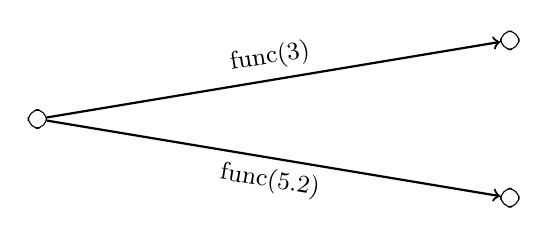
\begin{tikzpicture}[rectangle,rounded corners]
    \draw node (template) [draw] {\usebox{\codepiece}}
          node (templatea) [draw] at (6cm,+1cm) {\usebox{\codepiecea}}
          node (templateb) [draw] at (6cm,-1cm) {\usebox{\codepieceb}};
    \draw[->,thick] (template) -- (templatea) node [above,midway,sloped] {\small func(3)};
    \draw[->,thick] (template) -- (templateb) node [below,midway,sloped] {\small func(5.2)};
  \end{tikzpicture}
\end{frame}

\begin{frame}[fragile]
  \frametitlecpp[98]{Templates}
  \begin{block}{Arguments}
    \begin{itemize}
    \item can be a class,
    \item you can have several
    \item last ones can have a default value
    \end{itemize}
  \end{block}
  \begin{cppcode*}{}
    template<typename KeyType=int, typename ValueType=KeyType>
    struct Map {
      void set(const KeyType &key, ValueType value);
      ValueType get(const KeyType &key);
    }

    Map<std::string, int> m1;
    Map<float> m2;   // Map<float, float>
    Map<> m3;        // Map<int, int>
  \end{cppcode*}
\end{frame}

\begin{frame}[fragile]
  \frametitlecpp[98]{Templates implementation}
  \begin{cppcode*}{}
    template<typename KeyType=int, typename ValueType=KeyType>
    struct Map {
      void set(const KeyType &key, ValueType value);
      ValueType get(const KeyType &key);
    }

    template<typename KeyType, typename ValueType>
    void Map<KeyType, ValueType>::set
       (const KeyType &key, ValueType value) {
      ...
    }

    template<typename KeyType, typename ValueType>
    ValueType Map<KeyType, ValueType>::get
       (const KeyType &key) {
      ...
    }
  \end{cppcode*}
\end{frame}

\begin{frame}[fragile]
  \frametitle{Non-type template parameter \hfill \cpp98 / \cpp17 / \cpp20}
  \begin{block}{template parameters can also be a value}
    \begin{itemize}
    \item integral types, pointer, enums in \cpp98
    \item auto in \cpp17
    \item floats and literals in \cpp20
    \end{itemize}
  \end{block}
  \begin{cppcode*}{}
    template<unsigned int N> struct Polygon {
      Polygon(float radius);
      float perimeter() {return 2*N*sin(PI/N)*m_radius;}
      float m_radius;
    };
  \end{cppcode*}
\end{frame}

\begin{frame}[fragile]
  \frametitlecpp[98]{Templates}
  \begin{block}{Specialization}
    templates can be specialized for given values of their parameter
  \end{block}
  \begin{cppcode*}{}
    template<typename F, unsigned int N> struct Polygon {
      Polygon(F radius) : m_radius(radius) {}
      F perimeter() {return 2*N*sin(PI/N)*m_radius;}
      F m_radius;
    };

    template<typename F>
    struct Polygon<F, 6> {
      Polygon(F radius) : m_radius(radius) {}
      F perimeter() {return 6*m_radius;}
      F m_radius;
    };
  \end{cppcode*}
\end{frame}

\begin{frame}[fragile]
  \frametitlecpp[98]{The full power of templates}
  \begin{alertblock}{Exercise Time}
    \begin{itemize}
    \item go to code/templates
    \item look at the OrderedVector code
    \item compile and run playwithsort.cpp. See the ordering
    \item modify playwithsort.cpp and reuse OrderedVector with Complex
    \item improve OrderedVector to template the ordering
    \item test reverse ordering of strings (from the last letter)
    \item test order based on {\color{blue} \href{https://en.wikipedia.org/wiki/Taxicab_geometry}{Manhattan distance}} with complex type
    \item check the implementation of Complex
    \item try ordering complex of complex
    \end{itemize}
  \end{alertblock}
\end{frame}

\subsection[STL]{The STL}

\begin{frame}[fragile]
  \frametitlecpp[98]{The Standard Template Library}
  \begin{block}{What it is}
    \begin{itemize}
    \item A library of standard templates
    \item Everything you need, or ever dreamed of
      \begin{itemize}
      \item strings, containers, iterators
      \item algorithms, functions, sorters
      \item functors, allocators
      \item ...
      \end{itemize}
    \item Portable
    \item Reusable
    \item Efficient
    \end{itemize}
  \end{block}
  \pause
  \begin{alertblock}{Just use it}
    and adapt it to your needs, thanks to templates
  \end{alertblock}
\end{frame}

\begin{frame}[fragile,label=STLcode]
  \frametitlecpp[11]{STL in practice}
  \begin{cppcode*}{}
    #include <vector>
    #include <algorithm>

    std::vector<int> vi{5, 3, 4}; // initializer list
    std::vector<int> vr(3); // constructor taking int

    std::transform(vi.begin(), vi.end(),      // range1
                   vi.begin(),          // start range2
                   vr.begin(),          // start result
                   std::multiplies<int>()); // function

    for(auto n : vr) {
      std::cout << n << ' ';
    }
  \end{cppcode*}
\end{frame}

\begin{frame}[fragile]
  \frametitlecpp[98]{STL's concepts}
  \begin{block}{containers}
    \begin{itemize}
    \item a structure containing data
    \item with a given way of handling it
    \item irrespective of
      \begin{itemize}
      \item the data itself (templated)
      \item the memory allocation of the structure (templated)
      \item the algorithms that may use the structure
      \end{itemize}
    \item examples
      \begin{itemize}
      \item string
      \item tuple, list, vector, deque
      \item map, set, multimap, multiset, hash\_map, hash\_set, ...
      \item stack, queue, priority\_queue
      \end{itemize}
    \end{itemize}
  \end{block}
\end{frame}

\begin{frame}[fragile]
  \frametitlecpp[98]{STL's concepts}
  \begin{block}{iterators}
    \begin{itemize}
    \item generalization of pointers
    \item allowing iteration over some data
    \item irrespective of
      \begin{itemize}
      \item the container used (templated)
      \item the data itself (container is templated)
      \item the consumer of the data (templated algorithm)
      \end{itemize}
    \item examples
      \begin{itemize}
      \item iterator
      \item reverse\_iterator
      \item const\_iterator
      \end{itemize}
    \end{itemize}
  \end{block}
\end{frame}

\begin{frame}[fragile]
  \frametitlecpp[98]{STL's concepts}
  \begin{block}{algorithms}
    \begin{itemize}
    \item implementation of an algorithm working on data
    \item with a well defined behavior (defined complexity)
    \item irrespective of
      \begin{itemize}
      \item the data handled
      \item the container where data live
      \item the iterator used to go through data
      \end{itemize}
    \item examples
      \begin{itemize}
      \item for\_each, find, find\_if, count, count\_if, search
      \item copy, swap, transform, replace, fill, generate
      \item remove, remove\_if
      \item unique, reverse, rotate, random, partition
      \item sort, partial\_sort, merge, min, max
      \item lexicographical\_compare, iota, accumulate, partial\_sum
      \end{itemize}
    \end{itemize}
  \end{block}
\end{frame}

\begin{frame}[fragile]
  \frametitlecpp[98]{STL's concepts}
  \begin{block}{functions / functors}
    \begin{itemize}
      \item generic utility functions/functors
      \item mostly useful to be passed to STL algorithms
    \item implemented independently of
      \begin{itemize}
      \item the data handled (templated)
      \item the context (algorithm) calling it
      \end{itemize}
    \item examples
      \begin{itemize}
      \item plus, minus, multiply, divide, modulus, negate
      \item equal\_to, less, greater, less\_equal, ...
      \item logical\_and, logical\_or, logical\_not
      \item identity, project1st, project2nd
      \item binder1st, binder2nd, unary\_compose, binary\_compose
      \end{itemize}
    \end{itemize}
  \end{block}
\end{frame}

\againframe{STLcode}

\begin{frame}[fragile]
  \frametitlecpp[98]{STL in practice using \cpp98}
  \begin{cppcode*}{}
    #include <vector>
    #include <algorithm>

    std::vector<int> vi, vr(3);
    vi.push_back(5); vi.push_back(3); vi.push_back(4);

    std::transform(vi.begin(), vi.end(),      // range1
                   vi.begin(),          // start range2
                   vr.begin(),          // start result
                   std::multiplies<int>()); // function

    for(std::vector<int>::iterator it = vr.begin();
        it != vr.end();
        it++) {
      std::cout << *it << ' ';
    };
  \end{cppcode*}
\end{frame}

\begin{frame}[fragile]
  \frametitlecpp[98]{STL and functors}
  \begin{cppcode}
    // Finds the first element in a list that lies in
    // the range from 1 to 10.
    list<int> L;
    ...
    list<int>::iterator in_range =
      find_if(L.begin(), L.end(),
              compose2(logical_and<bool>(),
                       bind2nd(greater_equal<int>(), 1),
                       bind2nd(less_equal<int>(), 10)));

    // Computes sin(x)/(x + DBL_MIN) for elements of a range.
    transform(first, last, first,
              compose2(divides<double>(),
                       ptr_fun(sin),
                       bind2nd(plus<double>(), DBL_MIN)));
  \end{cppcode}
\end{frame}

\begin{frame}[fragile]
  \frametitlecpp[98]{Welcome to lego programming !}
  \begin{block}{}
    \pgfdeclareimage[height=0.5cm]{AtlasLego}{AtlasLego.jpg}
    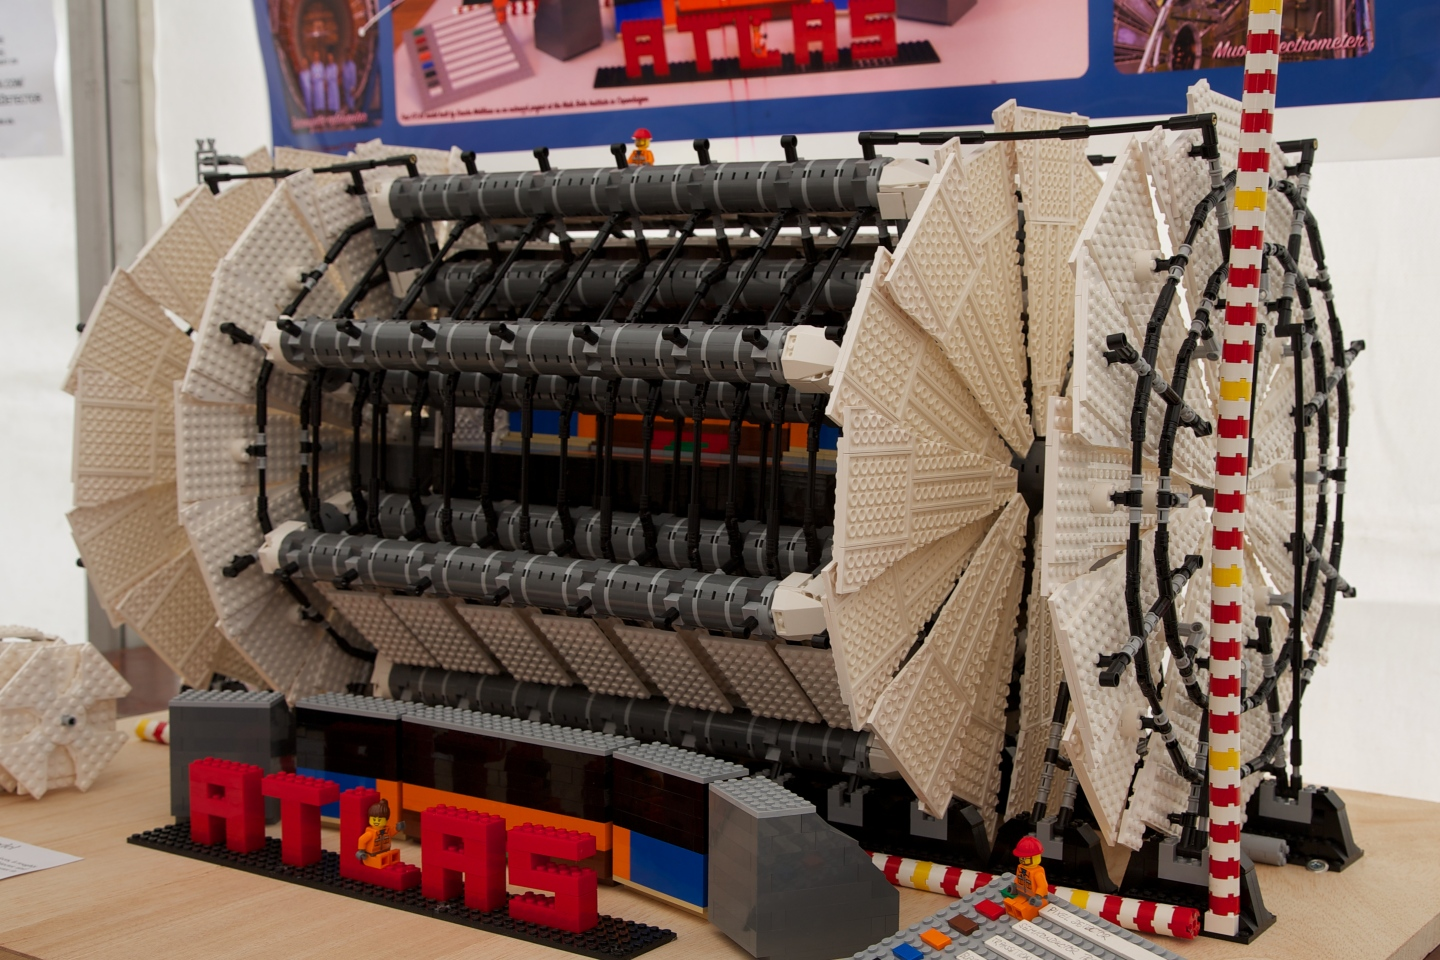
\includegraphics[width=\linewidth]{AtlasLego}
  \end{block}
\end{frame}

\begin{frame}[fragile]
  \frametitlecpp[98]{Using the STL}
  \begin{alertblock}{Exercise Time}
    \begin{itemize}
    \item go to code/stl
    \item look at the non STL code in randomize.nostl.cpp
      \begin{itemize}
        \item it creates a vector of ints at regular intervals
        \item it randomizes them
        \item it computes differences between consecutive ints
        \item and the mean and variance of it
      \end{itemize}
    \item open randomize.cpp and complete the ``translation'' to STL
    \item see how easy it is to reuse the code with complex numbers
    \end{itemize}
  \end{alertblock}
\end{frame}

\begin{frame}[fragile]
  \frametitlecpp[98]{Using the STL}
  \begin{alertblock}{Some last warning}
    You may find the STL quite difficult to use.
    \begin{itemize}
    \item template syntax is simply awful
    \item it is hard to debug (compilers spit out mostly garbage)
    \end{itemize}
    However, this has improved a lot with \cpp11 \\
    And will again in \cpp20 with concepts
  \end{alertblock}
\end{frame}

\begin{frame}[fragile]
  \frametitlecpp[11]{Loops and auto keyword with the STL}
  \begin{block}{Old way}
    \begin{cppcode*}{}
      std::vector<int> a = ...;
      int sum = 0;
      for (std::vector<int>::iterator it = v.begin();
           it != v.end(); it++) {
        sum += *it;
      }
    \end{cppcode*}
  \end{block}
  \pause
  \begin{block}{New way}
    \begin{cppcode*}{firstnumber=7}
      std::vector<int> v = ...;
      int sum = 0;
      for (auto a : v) { sum += a; }
    \end{cppcode*}
  \end{block}
  \pause
  \begin{exampleblock}{STL way}
    \begin{cppcode*}{firstnumber=10}
      std::vector<int> v = ...;
      int sum = std::accumulate(v.begin(), v.end(), 0);
    \end{cppcode*}
  \end{exampleblock}
\end{frame}

\subsection{More STL}

\begin{frame}[fragile]
  \frametitlecpp[17]{Some new STL types}
  \begin{block}{\texttt{std::optional}}
    \begin{itemize}
    \item manages an optional contained value
    \item contextually converted to bool
    \item useful for the return value of a function that may fail
    \end{itemize}
  \end{block}
  \begin{block}{\texttt{std::any}}
    \begin{itemize}
    \item a type-safe container for single values of any type
    \item the \texttt{any\_cast} function provides type-safe access
    \item and throws \texttt{std::bad\_any\_cast} for bad access
    \end{itemize}
  \end{block}
  \begin{block}{\texttt{std::variant}}
    \begin{itemize}
    \item a type-safe union
    \item \texttt{std::get} reads the value of the variant
    \item and throws \texttt{std::bad\_variant\_access} for bad accesses
    \end{itemize}
  \end{block}
\end{frame}

\begin{frame}[fragile]
  \frametitlecpp[11]{non-member begin and end}
  \begin{alertblock}{The problem in \cpp98}
    STL containers and arrays have different syntax for loop
    \vspace{-1mm}
    \begin{cppcode*}{}
      std::vector<int> v;
      int a[] = {1,2,3};
      for(auto it = v.begin(); it != v.end(); it++) {...}
      for(int i = 0; i < 3; i++) {...}
    \end{cppcode*}
  \end{alertblock}
  \pause
  \begin{block}{A new syntax}
    \begin{cppcode*}{firstnumber=5}
      for(auto it = begin(v); it != end(v); it++) {...}
      for(auto i = begin(a); i != end(a); i++) {...}
    \end{cppcode*}
  \end{block}
  \pause
  \begin{exampleblock}{Allowing the best syntax}
    \begin{cppcode*}{firstnumber=7}
      for(auto & element : v) {...}
      for(auto & element : a) {...}
    \end{cppcode*}
  \end{exampleblock}
\end{frame}

\begin{frame}[fragile]
  \frametitlecpp[17]{Structured Binding Declarations}
  Helps when using tuples as a return type.\\
  Automatically creates variables and ties them.
  \begin{alertblock}{\cpp14}
    \begin{cppcode*}{}
      void foo(std::tuple<int, double, long> tuple) {
        int a = 0;
        double b = 0.0;
        long c = 0;
        // a, b, c need to be declared first
        std::tie(a, b, c) = tuple;
    \end{cppcode*}
  \end{alertblock}
  \begin{exampleblock}{\cpp17}
    \begin{cppcode*}{firstnumber=7}
      void foo(std::tuple<int, double, long> tuple) {
      auto [ a, b, c ] = tuple;
    \end{cppcode*}
  \end{exampleblock}
\end{frame}

\subsection[$\lambda$]{Lambdas}

\begin{frame}[fragile]
  \frametitlecpp[11]{Function return type}
  \begin{block}{A new way to specify function's return type}
    \begin{cppcode*}{linenos=false}
      ReturnType fn_name(ArgType1, ArgType2);  //old
      auto fn_name(ArgType1, ArgType2) -> ReturnType;
    \end{cppcode*}
  \end{block}
  \pause
  \begin{block}{Advantages}
    \begin{itemize}
    \item Allows to simplify inner type definition
      \begin{cppcode*}{gobble=4}
        class TheClass {
          using inner_type = int;
          inner_type func();
        }
        TheClass::inner_type TheClass::func() {...}
        auto TheClass::func() -> inner_type {...}
      \end{cppcode*}
    \item C++14: ReturnType is not mandatory, compiler can deduce it
    \item will be used for lambdas
    \end{itemize}
  \end{block}
\end{frame}


\begin{frame}[fragile]
  \frametitlecpp[11]{Lambdas}
  \begin{block}{Definition}
    a lambda is a function with no name
  \end{block}
  \pause
  \begin{exampleblock}{Python example}
    \begin{pythoncode*}{}
      data = [1,9,3,8,3,7,4,6,5]

      # without lambdas
      def isOdd(n):
        return n%2 == 1
      print(filter(isOdd, data))

      # with lambdas
      print(filter(lambda n:n%2==1, data))
    \end{pythoncode*}
  \end{exampleblock}
\end{frame}

\begin{frame}[fragile]
  \frametitlecpp[11]{\cpp Lambdas}
  \begin{block}{Simplified syntax}
    \begin{cppcode*}{gobble=2}
      [] (args) -> type {
        code;
      }
    \end{cppcode*}
    The type specification is optional
  \end{block}
  \begin{exampleblock}{Usage example}
    \begin{cppcode*}{firstnumber=4,gobble=2}
      std::vector<int> data{1,2,3,4,5};
      for_each(begin(data), end(data),
               [](int i) {
                 std::cout << "The square of " << i
                           << " is " << i*i << std::endl;
               });
    \end{cppcode*}
  \end{exampleblock}
\end{frame}


\begin{frame}[fragile]
  \frametitlecpp[11]{Capture}
  \begin{block}{Python code}
    \begin{pythoncode*}{}
      increment = 3
      data = [1,9,3,8,3,7,4,6,5]
      map(lambda x : x + increment, data)
    \end{pythoncode*}
  \end{block}
  \pause
  \begin{block}{First attempt in \cpp}
    \begin{cppcode*}{firstnumber=4}
      int increment = 3;
      std::vector<int> data{1,9,3,8,3,7,4,6,5};
      transform(begin(data), end(data), begin(data),
                [](int x) { return x+increment; });
    \end{cppcode*}
  \end{block}
  \pause
  \begin{alertblock}{Error}
    \begin{minted}[gobble=6]{text}
        error: 'increment' is not captured
          [](int x) { return x+increment; });
                                     ^
    \end{minted}
  \end{alertblock}
\end{frame}

\begin{frame}[fragile]
  \frametitlecpp[11]{Capture}
  \begin{block}{Variable capture}
    \begin{itemize}
    \item external variables need to be explicitly captured
    \item captured variables are listed within initial []
    \end{itemize}
  \end{block}
  \pause
  \begin{exampleblock}{Example}
    \begin{cppcode*}{}
      int increment = 3;
      std::vector<int> data{1,9,3,8,3,7,4,6,5};
      transform(begin(data), end(data), begin(data),
                [increment](int x) {
                  return x+increment;
                });
    \end{cppcode*}
  \end{exampleblock}
\end{frame}

\begin{frame}[fragile]
  \frametitlecpp[11]{Default capture is by value}
  \begin{exampleblock}{Code example}
    \begin{cppcode}
      int sum = 0;
      std::vector<int> data{1,9,3,8,3,7,4,6,5};
      for_each(begin(data), end(data),
              [sum](int x) { sum += x; });
    \end{cppcode}
  \end{exampleblock}
  \pause
  \begin{alertblock}{Error}
    \begin{minted}[gobble=4]{text}
      error: assignment of read-only variable 'sum'
               [sum](int x) { sum += x; });
    \end{minted}
  \end{alertblock}
  \pause
  \begin{block}{Explanation}
    By default, variables are captured by value
  \end{block}
\end{frame}

\begin{frame}[fragile]
  \frametitlecpp[11]{Capture by reference}
  \begin{exampleblock}{Simple example}
    In order to capture by reference, add '\&' before the variable
    \begin{cppcode*}{}
      int sum = 0;
      std::vector<int> data{1,9,3,8,3,7,4,6,5};
      for_each(begin(data), end(data),
              [&sum](int x) { sum += x; });
    \end{cppcode*}
  \end{exampleblock}
  \pause
  \begin{exampleblock}{Mixed case}
    One can of course mix values and references
    \begin{cppcode*}{firstnumber=5}
      int sum = 0, offset = 1;
      std::vector<int> data{1,9,3,8,3,7,4,6,5};
      for_each(begin(data), end(data),
              [&sum, offset](int x) {
                sum += x + offset;
              });
    \end{cppcode*}
  \end{exampleblock}
\end{frame}

\begin{frame}[fragile]
  \frametitlecpp[11]{Capture all}
  \begin{block}{by value}
    \begin{cppcode*}{linenos=false}
      [=](...) { ... };
    \end{cppcode*}
  \end{block}
  \pause
  \begin{block}{by reference}
    \begin{cppcode*}{linenos=false}
      [&](...) { ... };
    \end{cppcode*}
  \end{block}
  \pause
  \begin{block}{exceptions}
    \begin{cppcode*}{linenos=false}
      [&, b](...) { ... };
      [=, &b](...) { ... };
    \end{cppcode*}
  \end{block}
\end{frame}

\begin{frame}[fragile]
  \frametitlecpp[11]{Lambdas rather than functors}
  \begin{exampleblock}{Example}
    \begin{cppcode*}{}
      auto build_incrementer = [](int inc) {
        return [inc](int value) { return value + inc; };
      };
      auto inc1 = build_incrementer(1);
      auto inc10 = build_incrementer(10);
      int i = 0;
      i = inc1(i);   // i = 1
      i = inc10(i);  // i = 11
    \end{cppcode*}
  \end{exampleblock}
  \begin{block}{How it works}
    \begin{itemize}
      \item build\_incrementer returns a function object
      \item this function's behavior depends on a parameter
      \item note how {\it auto} is useful here !
    \end{itemize}
  \end{block}
\end{frame}

\begin{frame}[fragile]
  \frametitlecpp[11]{{\texttt lambda}s makes the STL usable}
  \begin{block}{Before lambdas}
    \begin{cppcode*}{}
      struct Incrementer {
        int m_inc;
        Incrementer(int inc) : m_inc(inc) {}
        int operator() (int value) {
          return value + m_inc;
        };
      };
      std::vector<int> v{1, 2, 3};
      std::transform(begin(v), end(v), begin(v),
                     Incrementer(1));
      for (auto a : v) std::cout << a << " ";
      \end{cppcode*}
    \end{block}
\end{frame}

\begin{frame}[fragile]
  \frametitlecpp[11]{{\texttt lambda}s makes the STL usable}
  \begin{exampleblock}{With lambdas}
    \begin{cppcode*}{}
      std::vector<int> v{1, 2, 3};
      std::transform(begin(v), end(v), begin(v),
                     [](int value) {
                       return value + 1;
                     });
      for (auto a : v) std::cout << a << " ";
    \end{cppcode*}
  \end{exampleblock}
  \pause
  \begin{alertblock}{Conclusion}
    Use the STL !
  \end{alertblock}
\end{frame}

\begin{frame}[fragile]
  \frametitlecpp[11]{Lambdas}
  \begin{alertblock}{Exercise Time}
    \begin{itemize}
    \item go to code/lambdas
    \item look at the code (it's the solution to the stl exercise)
    \item use lambdas to simplify it
    \end{itemize}
  \end{alertblock}
\end{frame}

\subsection[RAII]{pointers and RAII}

\begin{frame}[fragile]
  \frametitlecpp[98]{Pointers : why they are error prone ?}
  \begin{exampleblock}{They need initialization
      \hfill \onslide<2->{\textcolor{orange}{\bf Seg Fault}}}
    \begin{cppcode*}{xleftmargin=20pt}
      char *s;
      try {
        callThatThrows();
        s = (char*) malloc(...);
        strncpy(s, ...);
      } catch (...) { ... }
      bar(s);
    \end{cppcode*}
  \end{exampleblock}
  \pause
  \pause
  \vspace{-2cm}
  \begin{exampleblock}{They need to be released
      \hfill \onslide<4->{\textcolor{orange}{\bf Memory leak}}}
    \begin{cppcode*}{xleftmargin=20pt}
      char *s = (char*) malloc(...);
      strncpy(s, ...);
      if (0 != strncmp(s, ...)) return;
      foo(s);
      free(s);
    \end{cppcode*}
  \end{exampleblock}
  \pause
  \pause
  \vspace{-2cm}
  \begin{exampleblock}{They need clear ownership
      \hfill \onslide<6->{\textcolor{orange}{\bf Who should release ?}}}
    \begin{cppcode*}{xleftmargin=20pt}
      char *s = (char*) malloc(...);
      strncpy(s, ...);
      someVector.push_back(s);
      someSet.add(s);
      std::thread t1(vecConsumer, someVector);
      std::thread t2(setConsumer, someSet);
    \end{cppcode*}
  \end{exampleblock}
\end{frame}

\begin{frame}[fragile]
  \frametitlecpp[98]{This problem exists for any resource}
  \begin{exampleblock}{For example with a file}
    \begin{cppcode*}{}
      try {
        FILE *handle = std::fopen(path, "w+");
        if (0 == handle) { throw ... }
        if (std::fputs(str, handle) == EOF) {
          throw ...
        }
        fclose(handle);
      } catch (...) { ... }
    \end{cppcode*}
  \end{exampleblock}
\end{frame}

\begin{frame}
  \frametitlecpp[98]{Resource Acquisition Is Initialization (RAII)}
  \begin{block}{Practically}
    Use object semantic to acquire/release resources
    \begin{itemize}
    \item wrap the resource inside an object
    \item acquire resource via object constructor
    \item release resource in destructor
    \item create this object on the stack so that it is automatically destructed when leaving the scope, including in case of exception
    \end{itemize}
  \end{block}
\end{frame}

\begin{frame}[fragile]
  \frametitlecpp[98]{RAII in practice}
  \begin{exampleblock}{File class}
    \begin{cppcode*}{}
      class File {
      public:
        File(const char* filename) :
          m_file_handle(std::fopen(filename, "w+")) {
          if (m_file_handle == NULL) { throw ... }
        }
        ~File() { std::fclose(m_file_handle); }
        void write (const char* str) {
          if (std::fputs(str, m_file_handle) == EOF) {
            throw ...
          }
        }
      private:
        FILE* m_file_handle;
      };
    \end{cppcode*}
  \end{exampleblock}
\end{frame}

\begin{frame}[fragile]
  \frametitlecpp[98]{RAII usage}
  \begin{exampleblock}{Usage of File class}
    \begin{cppcode*}{}
      void log_function() {
        // file opening, aka resource acquisition
        File logfile("logfile.txt") ;

        // file usage
        logfile.write("hello logfile!") ;

        // file is automatically closed by the call to
        // its destructor, even in case of exception !
      }
    \end{cppcode*}
  \end{exampleblock}
\end{frame}

\begin{frame}[fragile]
  \frametitlecpp[11]{std::unique\_ptr}
  \begin{block}{an RAII pointer}
    \begin{itemize}
    \item wraps a regular pointer
    \item has move only semantic
      \begin{itemize}
      \item the pointer is only owned once
      \end{itemize}
    \item in \textless{}memory\textgreater{} header
    \end{itemize}
  \end{block}
  \pause
  \begin{exampleblock}{Usage}
    \begin{cppcode*}{}
      Foo *p = new Foo{};  // allocation
      std::unique_ptr<Foo> uptr(p);
      std::cout << uptr.get() << " points to "
                << uptr->someMember << std::endl;
      void f(std::unique_ptr<Foo> ptr);
      f(std::move(uptr)); // transfer of ownership
      // deallocation when exiting f
      std::cout << uptr.get() << std::endl; // 0
    \end{cppcode*}
  \end{exampleblock}
\end{frame}

\begin{frame}[fragile]
  \frametitlecpp[11]{Quiz}
  \begin{exampleblock}{}
    \begin{cppcode*}{}
      Foo *p = new Foo{};  // allocation
      std::unique_ptr<Foo> uptr(p);
      void f(std::unique_ptr<Foo> ptr);
      f(uptr); // transfer of ownership
    \end{cppcode*}
    What do you expect ?
  \end{exampleblock}
  \pause
  \begin{alertblock}{Compilation Error}
    \begin{minted}{text}
test.cpp:15:5: error: call to deleted constructor
of 'std::unique_ptr<Foo>'
  f(uptr);
    ^~~~
/usr/include/c++/4.9/bits/unique_ptr.h:356:7: note:
 'unique_ptr' has been explicitly marked deleted here
 unique_ptr(const unique_ptr&) = delete;
 ^
    \end{minted}
  \end{alertblock}
\end{frame}

\begin{frame}[fragile]
  \frametitlecpp[14]{std::make\_unique}
  \begin{block}{}
    \begin{itemize}
    \item allocates directly a unique\_ptr
    \item no new or delete calls anymore !
    \end{itemize}
  \end{block}
  \pause
  \begin{exampleblock}{make\_unique usage}
    \begin{cppcode*}{}
      // allocation of one Foo object,
      // calling constructor with one argument
      auto a = std::make_unique<Foo>(memberValue);
      std::cout << a.get() << " points to "
                << a->someMember << std::endl;
      // allocation of an array of Foos
      // calling default constructor
      auto b = std::make_unique<Foo[]>(10);
      // deallocations
    \end{cppcode*}
  \end{exampleblock}
\end{frame}

\begin{frame}[fragile]
  \frametitlecpp[11]{RAII or raw pointers}
  \begin{block}{When to use what ?}
    \begin{itemize}
    \item Always use RAII for allocations
    \item You thus never have to deallocate !
    \item Use raw pointers for observer functions (or references)
      \begin{itemize}
      \item remember that unique\_ptr is move only
      \end{itemize}
    \end{itemize}
  \end{block}
  \pause
  \begin{exampleblock}{A question of ownership}
    \begin{cppcode*}{}
      unique_ptr<T> producer();
      void observer(const T&);
      void modifier(T&);
      void consumer(unique_ptr<T>);
      unique_ptr<T> pt{producer()};
      observer(*pt);            // Keep ownership
      modifier(*pt);            // Keep ownership
      consumer(std::move(pt));  // Transfer ownership
    \end{cppcode*}
  \end{exampleblock}
\end{frame}

\begin{frame}[fragile]
  \frametitlecpp[11]{unique\_ptr usage summary}
  \begin{block}{It's about lifetime management}
    \begin{itemize}
    \item Use unique\_ptr in functions taking part to the lifetime management
    \item Otherwise use raw pointers or references
    \end{itemize}
  \end{block}
\end{frame}

\begin{frame}[fragile]
  \frametitlecpp[11]{shared\_ptr, make\_shared}
  \begin{block}{shared\_ptr : a reference counting pointer}
    \begin{itemize}
    \item wraps a regular pointer like unique\_ptr
    \item has move and copy semantic
    \item uses internally reference counting
      \begin{itemize}
      \item "Would the last person out, please turn off the lights ?"
      \end{itemize}
    \item reference counting is thread-safe, therefore costly
    \end{itemize}
  \end{block}
  \begin{block}{make\_shared : creates a shared\_ptr}
    \begin{cppcode*}{}
      {
        auto sp = std::make_shared<Foo>(); // #ref = 1
        vector.push_back(sp);              // #ref = 2
        set.insert(sp);                    // #ref = 3
      } // #ref 2
    \end{cppcode*}
  \end{block}
\end{frame}

\begin{frame}[fragile]
  \frametitlecpp[98]{smart pointers}
  \begin{alertblock}{Exercise Time}
    \begin{itemize}
    \item go to code/smartPointers
    \item compile and run the program. It doesn't generate any output.
    \item Run with valgrind to check for leaks
      { \scriptsize
      \begin{minted}[gobble=6]{shell-session}
        $ valgrind --leak-check=full --track-origins=yes ./smartPointers
      \end{minted}
      }
    \item Go through {\ttfamily problem1()} to {\ttfamily problem3()} and fix the leaks using smart pointers.
    \item {\ttfamily problem4()} is the most difficult. Skip if not enough time.
    \end{itemize}
  \end{alertblock}
\end{frame}
